
\documentclass[review]{elsarticle}
\usepackage{hyperref}
\usepackage[margin=1in]{geometry}
\usepackage{graphicx}
\usepackage{amsmath}
\usepackage{placeins}
\usepackage{comment}
\usepackage{textcomp}
\usepackage{gensymb}
\usepackage{lineno}
\usepackage{color}
\usepackage{cleveref}
\usepackage{multicol}

\usepackage[utf8]{inputenc}
\usepackage[english]{babel}

\usepackage[dvipsnames]{xcolor}

%\journal{Journal of Nuclear Materials}
\bibliographystyle{elsarticle-num}

\begin{document}

\begin{frontmatter}

\title{An \textit{ab initio} molecular dynamics investigation of the thermophysical properties of molten NaCl-MgCl$_2$ }

\author[ncsu]{Kai Duemmler}
\author[inl]{Michael Woods}
\author[inl]{Toni Karlsson}
\author[inl]{Ruchi Gakhar\corref{qwe2}}
\cortext[qwe2]{Corresponding author}
\ead{ruchi.gakhar@inl.gov}
\author[ncsu,inl]{Benjamin Beeler\corref{qwe}}
\cortext[qwe]{Corresponding author}
\ead{bwbeeler@ncsu.edu}

\address[ncsu]{North Carolina State University, Raleigh, NC 27695}
\address[inl]{Idaho National Laboratory, Idaho Falls, ID 83415}
\date{\today}

\begin{abstract}
Molten salts have many applications in the nuclear and solar energy industries for thermal storage and heat transfer applications. However, there is a knowledge gap in molten salt thermophysical properties which hinders the technical readiness level of molten salt applications, especially in the nuclear industry. A common method of investigating new materials is through \textit{ab initio} Molecular Dynamics (AIMD) simulations which is an effective tool to investigate structural and thermophysical properties at realistic temperatures. NaCl-MgCl$_2$ is an inexpensive salt that is a good candidate for use as a heat transfer medium in solar power applications or in the secondary loop of a nuclear reactor. In this article, the thermophysical properties of NaCl-MgCl$_2$ are computed via AIMD calculations to supplement the limited experimental studies in the literature. A wide range of compositions and temperatures for the pseudo-binary NaCl-MgCl$_2$ were used to calculate the density, heat capacity, compressibility, enthalpy of mixing, and volumetric thermal expansion coefficient. AIMD is shown to accurately model the densities of molten NaCl-MgCl$_2$ as there is good agreement with the available literature. Observed a transition to a monotonic increase of the density with respect to MgCl$_2$ composition occurs above 1100 K. The heat capacity values increase uniformly with respect to concentration of MgCl$_2$ at a rate of 2.85 J/mol-K per 10 mol\% of MgCl$_2$. Select thermophysical properties are fit to a Redlich-Kister expansion for utilization in multiphysics simulations. 
\end{abstract}

\end{frontmatter}

%\begin{multicols}{2}

\section{Introduction}
Molten salts have historically been used as a processing medium for catalysis \cite{JIN20202382, HU20204244} or metal production \cite{Zhu2014, VAHIDI2018178}, as well as different pyroprocessing methods for treating used nuclear fuel \cite{CHOI2015572, osti_22107867}. Today there is a focus on using molten salts as a thermal energy storage system or as a heat transfer medium in both the solar and nuclear industries. In the nuclear industry, there are two designs for Generation IV molten salt reactors (MSRs). The first is a solid-fueled, salt-cooled design where the salt is only a heat transfer medium and the fuel is a solid \cite{doi:10.13182/NSE90-374}. The second is the liquid-salt-fueled design where the salt mixture is the fuel and contains uranium, plutonium, and/or thorium salts \cite{doi:10.1080/00295450.2019.1586372}. In both cases, the salt will serve as a heat transfer medium to remove heat out of the primary loop and into the secondary loop \cite{gakhar2021molten}. There are several advantages to using molten salts as a heat transfer medium compared to pressurized water, including requiring little to no pressurization, which is an inherent safety advantage \cite{leblanc2017integral}. Molten salts also have favorable properties which make them good candidates for removing heat, including their volumetric heat capacity, viscosity, and thermal conductivity. They can also have large moderating ratios and low neutron capture cross sections when considering their use as a fuel salt \cite{williams2006assessment}.

One popular candidate salt mixture for both thermal storage media and for use as a heat transfer fluid is NaCl-MgCl$_{2}$. It has been suggested for use in concentrated solar power plants and as a coolant in the heat-transfer loop in advanced nuclear reactor designs due to its wide operating temperature range, lower cost \cite{williams2008evaluation}, and thermal stability \cite{XU2020568,williams2006assessment}. Experimental studies on the NaCl-MgCl$_2$ molten salt in the literature are limited due to the complexity of handling molten salts at extreme temperatures. These property measurements can be very sensitive to any impurities present in the salt, including oxygen absorbed due to the hygroscopic nature of the salt \cite{bell2019corrosion}. In addition, some salts present other hazards which make handling and measurements difficult, such as the toxicity hazards of beryllium containing salts and the radioactive concerns of salts containing actinides. Due to both the complexity of molten salt experiments and the lack of interest in molten salt applications from the nuclear community until recently, there is a knowledge gap in the thermophysical properties of many molten salts. Research of NaCl-MgCl$_{2}$ has primarily focused only on the eutectic composition, with investigations reporting the eutectic temperature, thermal stability, and heat capacity \cite{MOHAN2018156}. There have been a select number of investigations that have spanned the full compositional spectrum, but these were limited to a narrow temperature range and only explored the density, surface tension, electrical conductance, and viscosity \cite{Janz1988}.

Molecular simulation, both classical and \textit{ab initio} (sometimes called first principles methods) molecular dynamics, is a valuable tool to scope the properties of molten salt mixtures. The advantage of using classical molecular dynamics (CMD) is that it can be used to describe systems of up to millions of atoms evolving over nanoseconds, but it is limited by the existing interatomic potentials and the accuracy of their parameterization. This limits their application to newer molten salts that have not been parameterized, or temperature ranges that have not been accounted for. The advantages of \textit{ab initio} molecular dynamics (AIMD) is that it removes the need for interatomic potentials by calculating the energy from first principles from the electron interactions. As a consequence, this is more computationally expensive then CMD, restricting the number of atoms to a few hundred and the timescale to picoseconds, but provides increased accuracy. Many of the available studies for NaCl-MgCl$_{2}$ in literature are either CMD or AIMD. These studies supplement the missing experimental information in the literature. Xu et al. studied the pseudobinary salt phase transition through AIMD \cite{XU2020568}. Takagi and Tomita used CMD to study the structural properties, such as the structure factor, first peak distances, and the pair correlation function \cite{takagi1993structure}. Molecular dynamics is a powerful tool to study the influence of impurities in molten salts as shown by Li et al. \cite{li2020insight} in the MgCl$_{2}$-NaCl-KCl system through the use of AIMD. AIMD has been used on several other molten salt systems including LiCl-KCl \cite{Duemmler2021,Bengston2014,Song2017}, FLiNaK\cite{NAM2014148}, and FLiBe\cite{NAM2014148}. 

In this investigation, AIMD is employed to study the full compositional spectrum of binary NaCl-MgCl$_{2}$ from 800 K to 1300 K based on the contours of the phase diagram. First, the bond distances are calculated from the radial distribution function, then the densities are calculated along with the compressibility, isobaric heat capacity, enthalpy of mixing, and the volumetric thermal expansion. These are all important parameters that are needed in the design of molten salt cooling loops. Along with these properties, a study of the ideal mixing law is conducted and the deviation is interpreted with a Redlich-Kister expansion formalism \cite{redlich1948}. This is the most complete exploration of thermophysical properties for the NaCl-MgCl$_2$ system, and utilizes a previously novel dispersion formalism that improves property prediction. 

\section{Computational Methods}

\subsection{Ab Initio Molecular Dynamics}
This study employs AIMD through the Vienna \textit{ab initio} Simulation Package (VASP) \cite{Kresse1993,Kresse1996,Kresse1996a}. Six unique compositions of NaCl-MgCl$_{2}$ were studied: 0\%, 20\%, 42.7\% (eutectic) \cite{FTsalt}, 60\%, 80\%, and 100\% MgCl$_{2}$ (compositions given in molecular percent). The size of the systems was approximately 200 atoms, with small variations due to compositional variance. The temperature range was 800 to 1300 K following the contours of the phase diagram \cite{FTsalt} so that only molten NaCl-MgCl$_{2}$ compositions in the liquid state were studied. To account for the dispersion interaction within the molten NaCl-MgCl$_{2}$, the vdW-DF2 Van der Waals functional \cite{Dion2004} was employed as it has been shown to follow the density trend across the full computational spectrum in other molten salts \cite{Duemmler2021}. Additional verification of the applicability of the vdW-DF2 functional was performed in this investigation, with comparisons to the DFT-D3 \cite{grimm2010} method and to density functional theory (DFT) without dispersion. All simulations were carried out in the canonical (NVT) ensemble, where the temperature was controlled through a Langevin thermostat with a friction coefficient of 10 ps$^{-1}$ for all atoms. The timestep employed was 2.5 femtoseconds. The electronic optimization criterion was 10$^{-4}$ eV and the cutoff energy was 300 eV. A 1$\times$1$\times$1 k-point mesh was implemented at the gamma point, which has previously been demonstrated to be sufficient in the literature \cite{Bengston2014,Song2017}.

The simulation system was created with the PACKMOL package \cite{martinez2009} which randomly places molecules or atoms within a confined space based on certain geometric constraints. First, the initial systems were equilibrated at 2000 K to allow for mixing and to confirm that the system was a liquid through analysis of the radial distribution function. Subsequently, the systems were quenched to their corresponding target temperatures and then further equilibrated. Following this, the equilibrium volume can be determined by sampling the pressure with respect to volume. Detailed explanation of the method can be found in a previous study \cite{Duemmler2021}. 

The bond length can be calculated from the radial distribution functions by finding the distance at which the first peak occurs for the corresponding atom interaction. The radial distribution functions were created through the \textit{vasppy} python package with the default smearing which applies a Gaussian kernel to the data with a sigma parameter of 0.1. The bulk modulus can be calculated from the change in pressure with respect to volume as shown below in Eq. \ref{eq:bulk modulus},
\begin{equation}
\label{eq:bulk modulus}
K = -V {(\frac{dP}{dV})}_{P=0}
\end{equation} where $K$ is the bulk modulus, $V$ is the volume, and $P$ is the pressure. Compressibility of a liquid is the inverse of the bulk modulus, as shown in Eq. \ref{eq:compressibility}. 
\begin{equation}
\label{eq:compressibility}
\beta = \frac{1}{K}
\end{equation}
To ensure comparable data across temperature and composition, the pressure ranges for each system (volume, composition, and temperature) were limited from 7 to -2 kBar. Each system contained at least five unique volumes and each volume contained at least five distinct simulations. The same formulation was employed to determine the equilibrated energy, in that a pressure versus energy curve was constructed and the energy at a pressure of zero is identified as the equilibrated energy of the system. 


The isobaric heat capacity was calculated by first applying a linear fit to the total energy over the corresponding temperature range for each composition on the NaCl-MgCl$_2$ system. The isobaric heat capacity value is the slope of the linear fit to the data and is valid for the temperature range studied. It is possible to calculate the enthalpy of mixing from the potential energy of the mixed system and the two binary salts as shown in Eq. \ref{eq:enthalpy},
\begin{equation}
 \label{eq:enthalpy}
 \Delta H^{mix} = \frac{E_{AB}}{M_{AB}} - \frac{x_A E_A}{M_A} - \frac{x_B E_B}{M_B}
\end{equation}
where M$_i$ is the number of molecules in that respective system, E$_A$ and E$_B$ are the potential energies of the reference systems, NaCl and MgCl$_2$, E$_{AB}$ is the potential energy of the mixed system, and $x_A$ and $x_B$ are the mole fraction of the two respective reference salts in the mixture. The volumetric coefficient of thermal expansion can be defined as the linear fit to volume as a function of temperature divided by a reference volume as seen in Eq. \ref{eq:CTE}, where $V$ is the volume of the system at temperature $T$ and $V_r$ is the reference volume at the lowest temperature for each composition.

\begin{equation}
 \label{eq:CTE}
   \alpha = \frac{1}{V_{r}}\frac{dV}{dT}
\end{equation}

\subsection{Redlich-Kister model}
The Redlich-Kister model describes the density with respect to composition as a summation of the ideal mixing density and an excess density, as in Eq. \ref{eq:density},
\begin{equation}
 \label{eq:density}
   \rho_{mix} = \rho_{id} + \rho_{ex}
\end{equation}where $\rho_{mix}$ is the density at a given composition and temperature, $\rho_{id}$ is the density calculated from the ideal mixing law, and $\rho_{ex}$ is the excess density that can be modeled by the Redlich-Kister expansion. The ideal mixing density can be determined either from a weighted molar average of the densities \cite{guo1989density,cooper1991densities} or weighted molar volumes which can then be converted to densities \cite{agca2022,chrenkova2003density,mlynarikova2017volume}. The latter approach, which is the the additive behavior approach, was used here and is shown in Eq. \ref{eq:mixing}.
\begin{equation}
  \label{eq:mixing} 
     \rho_{id} = \frac{\sum_i x_iM_{i}}{\sum_i x_iV_{i}}
\end{equation}
where $x_i$ is the atom fraction and $M$ and $V$ are the formula mass and volume per molecule for NaCl and MgCl$_2$. The Redlich-Kister expansion \cite{redlich1948} is designed to show the excess properties from a non-ideal density through multiple components and can be defined in Eq. \ref{eq:RK},

\begin{equation}
  \label{eq:RK}
     \rho_{ex} = x(1-x) \sum_{n-1}^{N} L_n(2x-1)^{n-1}
\end{equation}
where in this case $x$ is the concentration of MgCl$_{2}$ in mol\% and $N$ is the total number of $L_{N}$, which is a linear temperature-dependent function shown in Eq. \ref{eq:Ln} \cite{agca2022},
\begin{equation}
  \label{eq:Ln}
     L_n = A_n+B_nT
\end{equation}
where $A_n$ and $B_n$ are fitting parameters and $T$ is the temperature. This formalism can be applied to other properties beyond the density, such as the enthalpy of mixing. In this work, the order of the Redlich-Kister expansion is denoted by $n-1$, e.g., for $n=2$ the Redlich-Kister expansion has an order of one.
\FloatBarrier
\section{Results and Discussion}

\subsection{Evaluation of van der Waals dispersion interactions}

The van der Waals (vdW) force plays a fundamental role in determining the structure and properties of ionic liquids. The traditional exchange correlations (local density approximation and generalized gradient approximation) do not account for dispersion forces founds in ionic liquids. Due to this, either a dispersion term needs to be considered for evaluation of energies and forces or the exchange correlation itself needs to account for dispersive forces. The influence of different vdW corrections on molten salts has been shown for LiCl-KCl \cite{Duemmler2021}, for example. In this study, the vdW-DF2 van der Waals functional \cite{Dion2004} is compared against the generalized gradient approximation of Perdew-Burke-Ernzerhof (PBE) \cite{PBE1996} and the DFT-D3 \cite{grimm2010} dispersion correction. The PBE method does not take into account dispersion interactions that can be found in ionic liquids like molten salts and often leads to an underprediction of the density. The DFT-D3 dispersion correction builds upon the prior DFT-D methods by adding an eighth-order atom-pairwise dispersion term that is geometry-dependent \cite{grimm2010}. The densities of the NaCl and the MgCl$_2$ systems at 1100 K evaluated with the vdW-DF2, PBE, and DFT-D3 formalisms are shown in Table \ref{table:functional}. It can be observed that the vdW-DF2 functional is the best approach for calculation of the densities of the binary salts, while the non-dispersion PBE functional under-predicts the density, and the DFT-D3 dispersion correction over-predicts the densities. It should be noted that the correct choice of dispersion interaction should be identified for each system and the dispersion functional chosen here may not always be the most appropriate choice. All subsequent results presented are calculated with the vdW-DF2 functional.
\begin{table}[h]
\centering
\caption{Density values for NaCl and MgCl$_2$ for different dispersion functionals at 1100 K compared to experimental literature value at 1073 K \cite{grjotheim1971} }
\begin{tabular}{|c|c|c|}
\hline
Method & NaCl (g cm$^{-3}$) & MgCl$_2$ (g cm$^{-3}$) \\
\hline

vdw-DF2	& 1.557       & 1.656\\
PBE	  & 1.397	      & 1.487\\
DFT-D3	& 1.776	      & 1.959\\
Exp	  & 1.56	      & 1.66\\

\hline
\end{tabular}
\label{table:functional}
\end{table}

\FloatBarrier

\subsection{Structural Properties}

AIMD simulations can provide structural information about the system that is being studied. An illustration of this is shown below in Fig. \ref{fig:rdf} which shows the radial distribution function for the eutectic composition of NaCl-MgCl$_2$ at 1100 K (Fig. \ref{fig:rdf}A) and the radial distribution function form MgCl$_2$ at 1000 K (Fig. \ref{fig:rdf}B). From this figure it is possible to extract the bond distance for each ion pair interaction. It can be seen in Fig. \ref{fig:rdf} that after the first peak the radial distribution function quickly approaches 1, which is the expected behavior for a liquid. The bond length can be determined experimentally through neutron diffraction, as shown by Biggin et al. for MgCl$_2$ at 998.15 K \cite{biggin1984structures}. Biggin et al. found the bond lengths to be 2.42 $\pm$ 0.03 \r{A} for the Mg-Cl bond, 3.81 $\pm$ 0.05 \r{A} for the Mg-Mg bond, and  3.56 $\pm$ 0.04\r{A} for the Cl-Cl bond. Our study slightly underpredicts the Mg-Cl bond with a value of 2.39 \r{A}, while overpredicting the values for the like ion bonds of Mg-Mg and Cl-Cl with values of 4.13 and 3.73 \r{A}, respectively. Overall there is good agreement with experimental values with an average difference of 4.52\%. There are no experimental studies for the pseudo-binary system so they are compared to a CMD study at 1100 K from Takagi and Tomita \cite{takagi1993structure}. When comparing our NaCl-80\%MgCl$_2$ to Takagi and Tomita's NaCl-75\%MgCl$_2$, the average difference was 5.99\% when only comparing the Cl-Cl, Mg-Mg, and Mg-Cl bond distance. The CMD study did not report the bonds with Na. For the comparison of NaCl-20\%MgCl$_2$ against Takagi and Tomita's NaCl-23\%MgCl$_2$, the average difference was 12.07\%. Overall there is good agreement with experimental values for MgCl$_2$ and comparable results to the CMD study for NaCl-MgCl$_2$.

\begin{figure}[h]
 \centering
 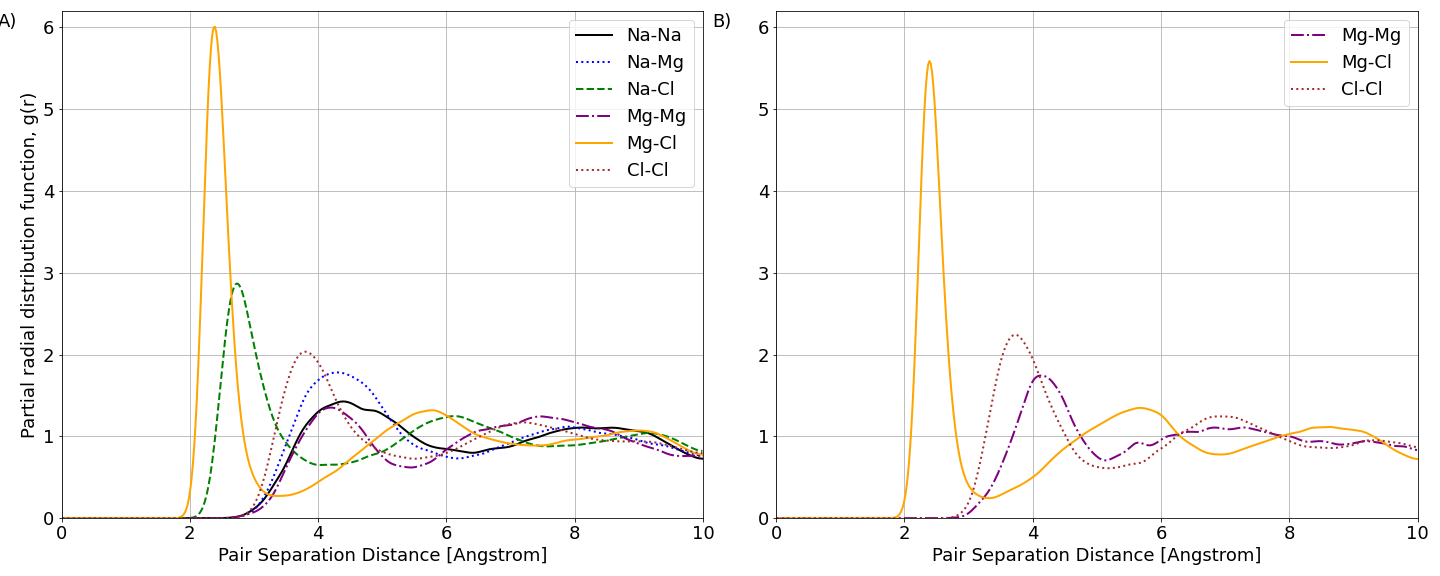
\includegraphics[width=0.9\textwidth]{images/rdf_from_vasppy.png} 
 \caption{A) The radial distribution function for the eutectic composition of NaCl-MgCl$_2$ at 1100 K. B) The radial distribution function for MgCl$_2$ at 1000 K.}
 \label{fig:rdf}
\end{figure} 

% \begin{table}[h]
% \centering
% \caption{Bond distance for MgCl$_2$ at 1000 K compared to x-ray diffraction \cite{biggin1984structures}.}

% \begin{tabular}{|c|c|c|}

% \hline
% Bond & AIMD (\r{A})  & XRD (\r{A})\\
% \hline

% Mg-Cl  &  2.3  &  2.42 \pm 0.03 \\
% Mg-Mg  &  4.1  &  3.81 \pm 0.05 \\
% Cl-Cl  &  3.9  &  3.56 \pm 0.04 \\

% \hline
% \end{tabular}
% \label{table:bond}
% \end{table}

\subsection{Thermophysical Properties}
The density of the NaCl-MgCl$_2$ system is shown in Fig. \ref{fig:density} as a function of both composition and temperature. There is a comparison to literature at 1073 K with Grjotheim et al. \cite{grjotheim1971} and at 1100 K with Janz \cite{Janz1988}. The density generally increases with increasing MgCl$_2$, as would be expected given the lower density of NaCl compared to MgCl$_2$. Interestingly, below 1200 K the density of NaCl-80\%MgCl$_2$ is higher than pure MgCl$_2$, shown in the data points at 1000 K and 1100 K. These AIMD results show very good agreement with the literature values as the AIMD results fall in between the two sets of experimental data. This includes the trend where the density at NaCl-80\%MgCl$_2$ is higher than pure MgCl$_2$ \cite{grjotheim1971}. The transition to monotonic increasing of density at temperatures above 1100 K has not been identified previously. Note that the experimental values do not report an estimated measurement error. The tabulated values for density and the other properties can be located in Appendix A.
\begin{figure}[h]
 \centering
 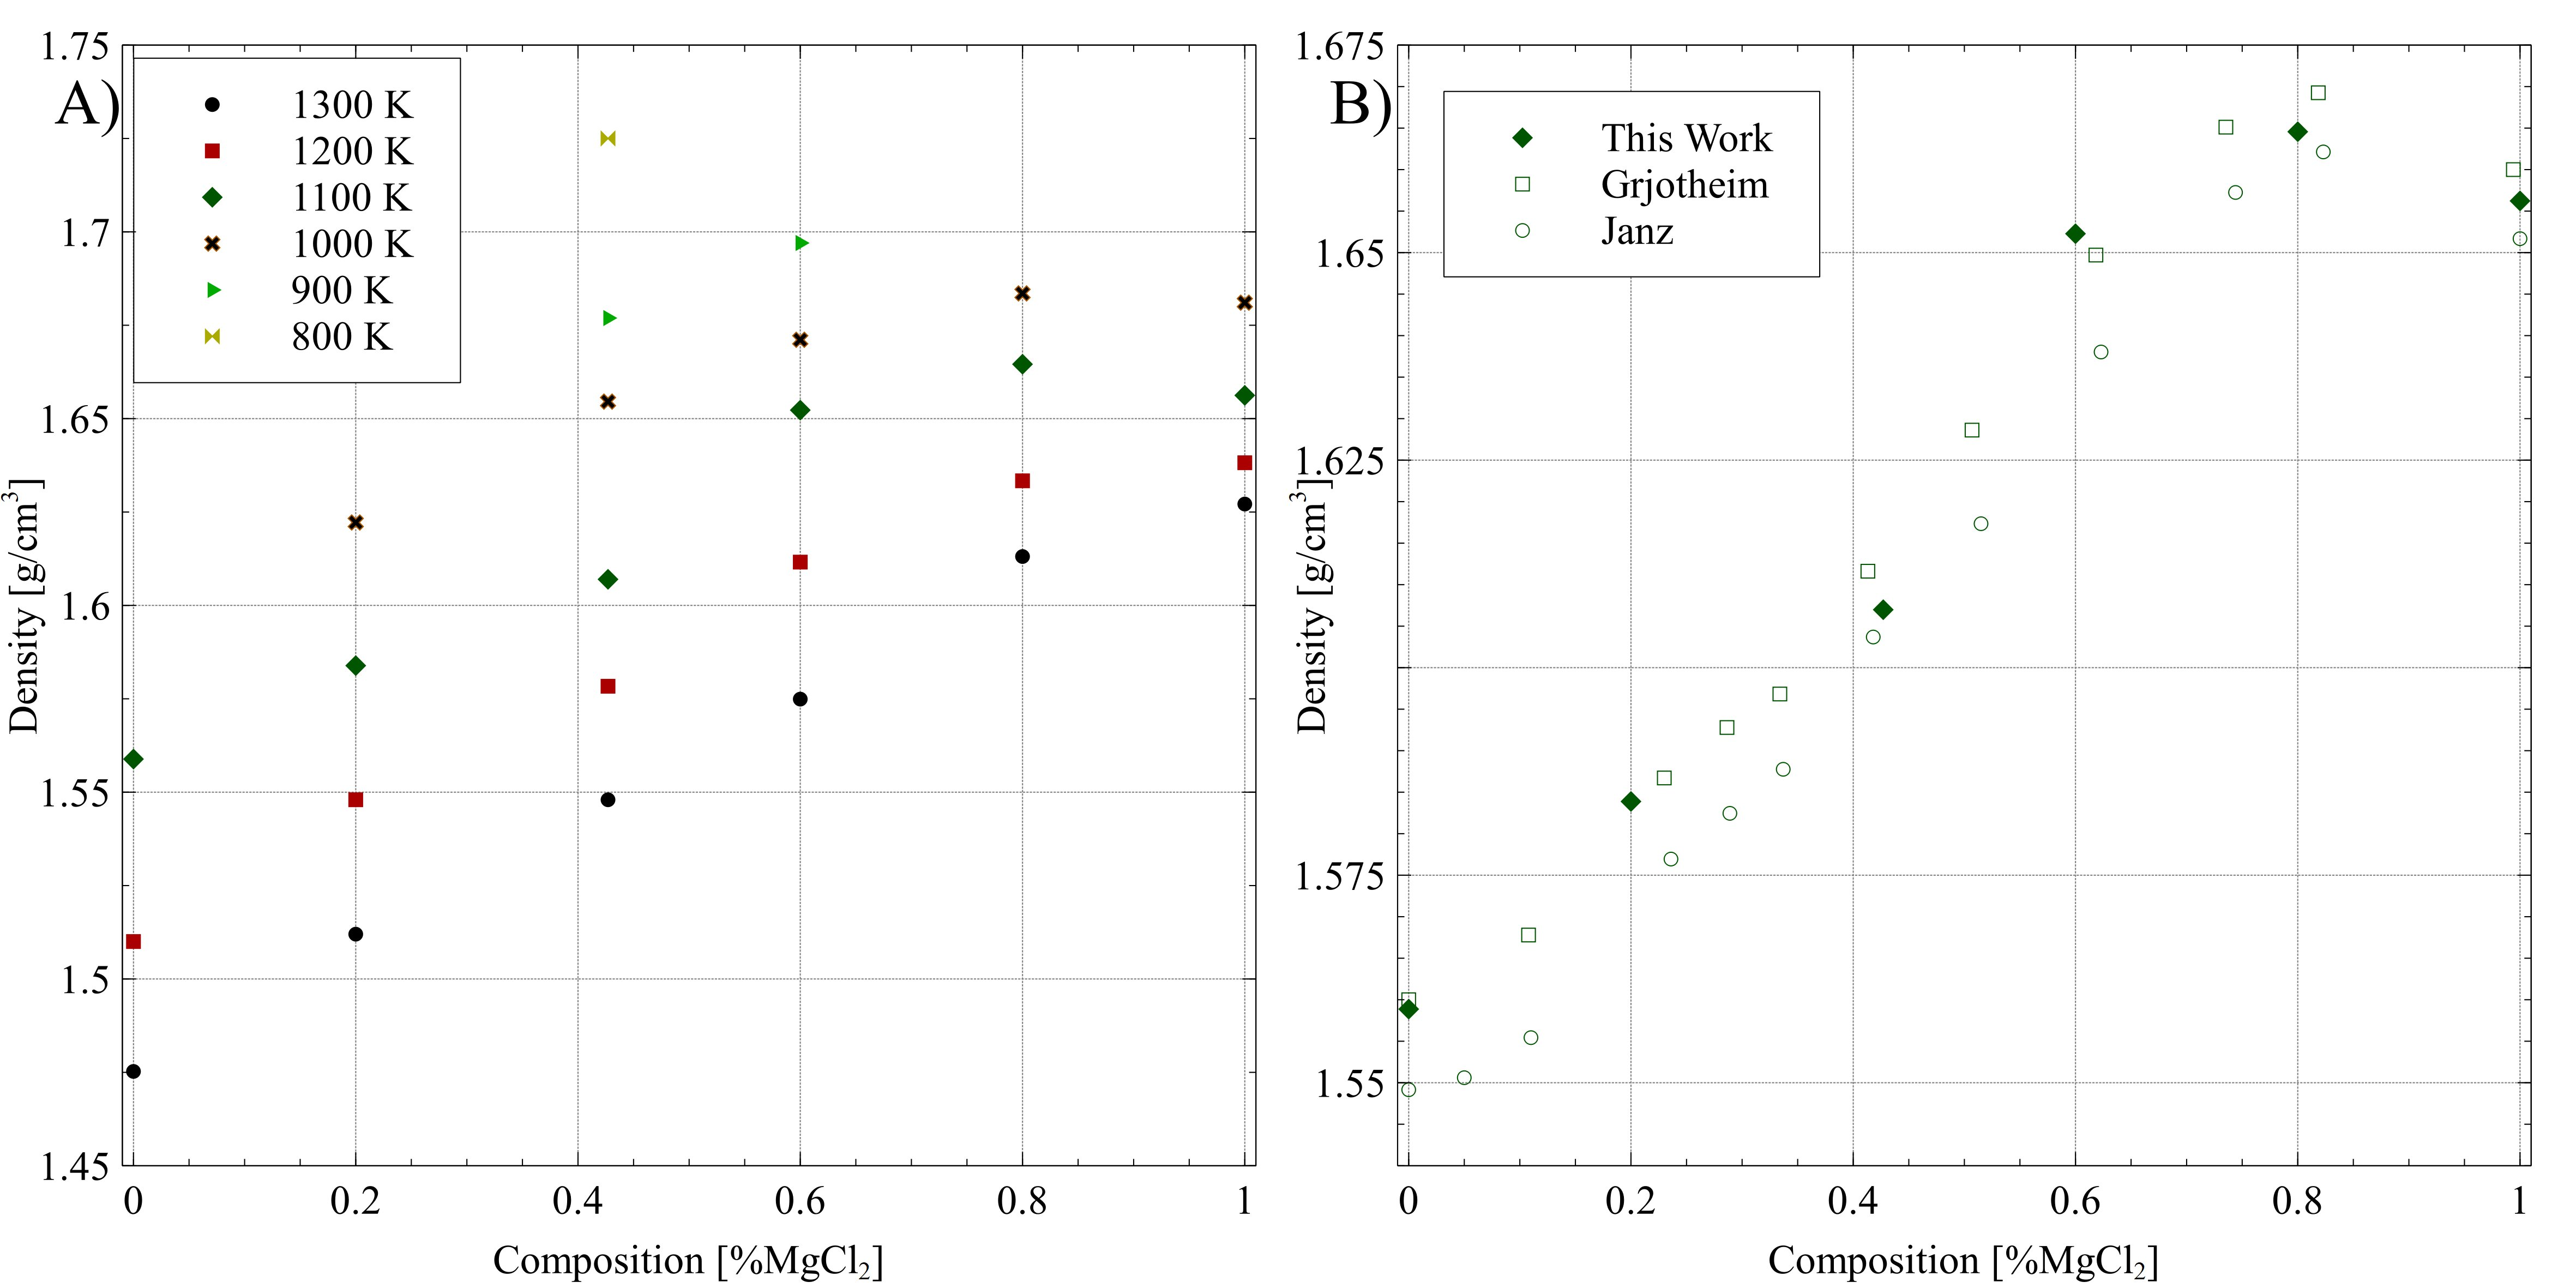
\includegraphics[width=1.0\textwidth]{images/density_combined_figures.jpg} 
 \caption{A) Densities for NaCl-MgCl$_2$ as a function of composition. B) Comparison from literature is at 1073 K (Grjotheim) \cite{grjotheim1971} and 1100 K (Janz) \cite{Janz1988}}
 \label{fig:density}
\end{figure} 

The density of a pseudo-binary mixture can be estimated from the densities of the two binary salts (NaCl and MgCl$_2$) utilizing either an ideal solution approximation or a modification of the ideal solution. An ideal solution-based compositional density is calculated below and shown as the solid lines in Fig. \ref{fig:density_mixing}. The ideal mixing law interpolates the densities between the two end points, which can be a reasonable approximation for some molten salts. This is not the case for NaCl-MgCl$_2$ as 80\% MgCl$_2$ has the highest density among the compositions analyzed at 1100 K. This creates a large error for compositions richer in MgCl$_2$ than the eutectic composition if the ideal mixing law is utilized to approximate densities. As seen in Fig. \ref{fig:density_mixing}, as the temperature increases, the density of MgCl$_2$ decreases the least of all compositions, resulting in a larger density of MgCl$_2$ than 80\% MgCl$_2$ at high temperatures. This suggests that at temperatures above 1300 K the ideal mixing law may be a good model for the density. The Redlich-Kister expansion was added to the ideal mixing law to correct for the deviation from ideal mixing and a first order expansion was sufficient to provide accurate fitting. The parameters for the first order expansion are shown in Table \ref{table:RK_parameters} and the corrected fit can be seen in Fig. \ref{fig:density_mixing} as the dotted lines, which shows good agreement with the simulated density with an average percent difference of 0.26\% (excluding endpoints, which are exactly reproduced). 

\begin{figure}[h]
 \centering
 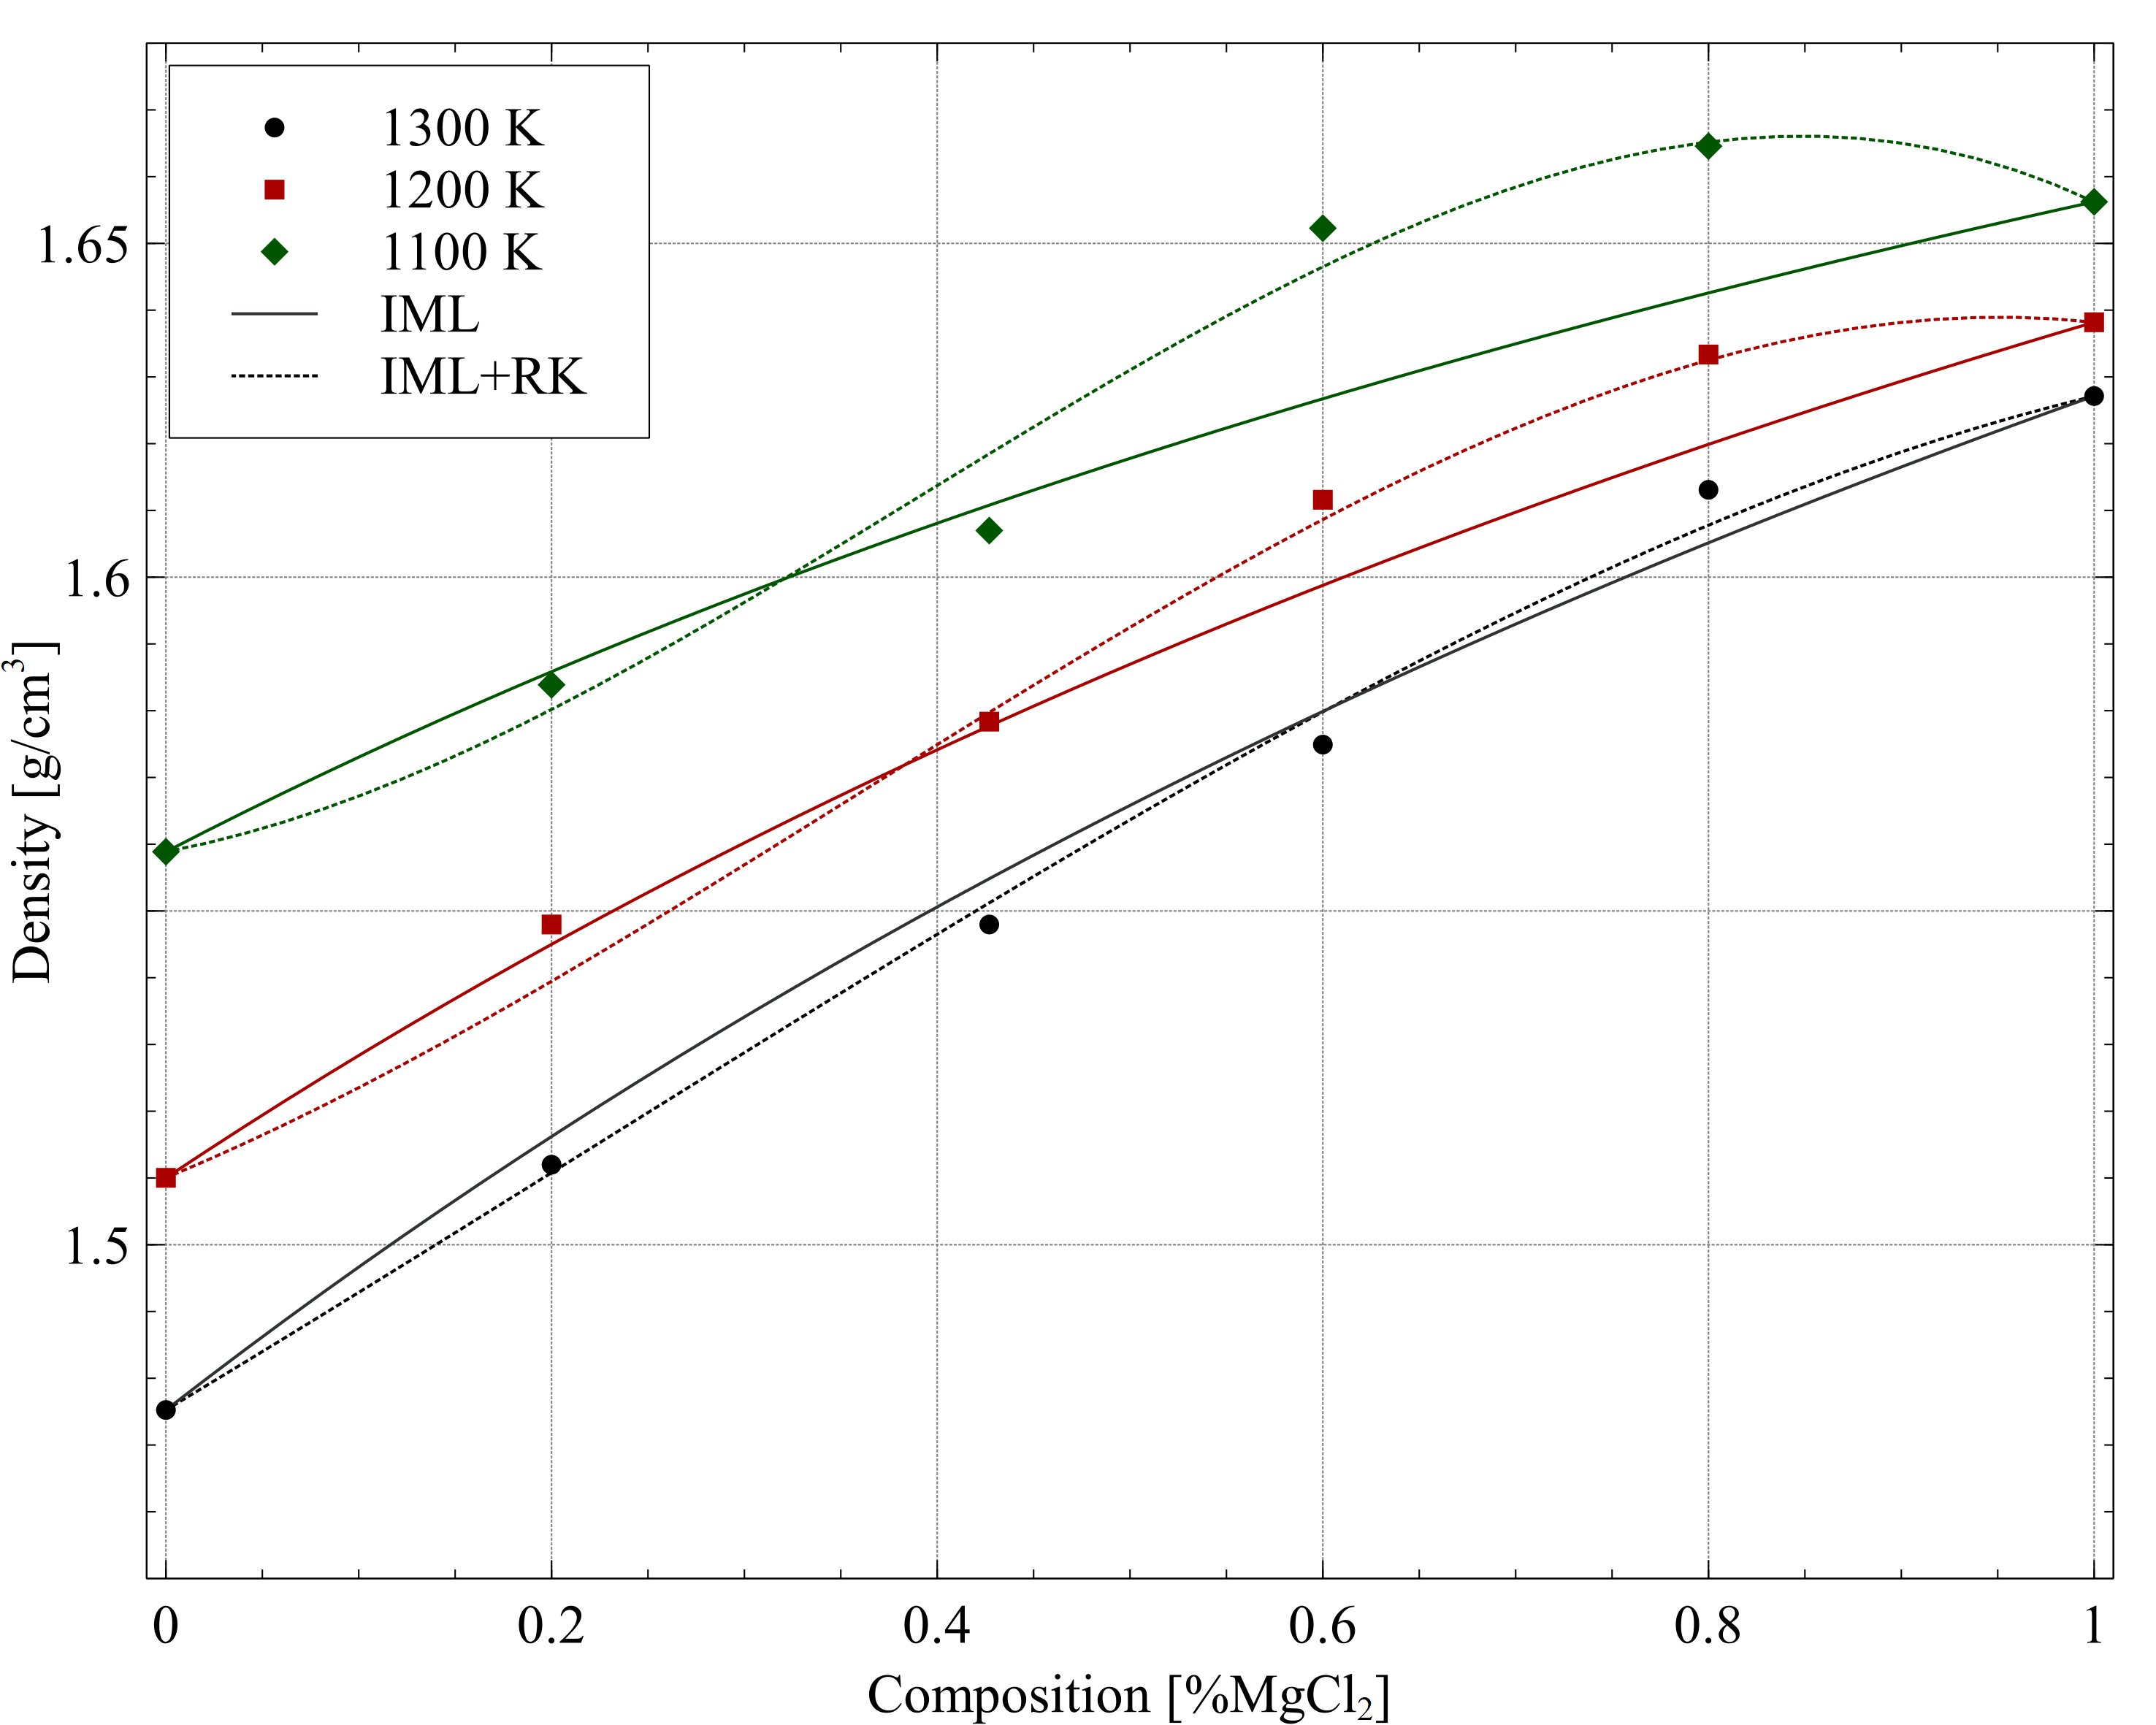
\includegraphics[width=0.8\textwidth]{images/density_mixing.jpg} 
 \caption{Densities for NaCl-MgCl$_2$ as a function of composition compared against the ideal mixing law (IML) and the IML with the Redlich-Kister expansion (IML+RK).}
 \label{fig:density_mixing}
\end{figure} 

\begin{table}[]
\centering
\caption{Redlich-Kister expansion parameters for the density of the NaCl-MgCl$_2$ system from 1100 K to 1300 K.}
\begin{tabular}{|c|c|c|}
\hline
Parameter &1 & 2 \\
\hline
A	& 0.39176716      & 0.72629546\\
B	  & -0.00030802	      & -0.00052639\\
\hline
\end{tabular}
\label{table:RK_parameters}
\end{table}

\FloatBarrier

The compressibility as a function of composition and temperature is shown in Fig. \ref{fig:compressibility}. The linear fits are displayed to illustrate the general trends of the data and do not suggest an actual linear trend for the data. Compressibility displays significantly greater scatter than the density, however, general trends can still be extracted. As the temperature increases, the compressibility tends to increase. The compressibility of the system has a slight positive relationship with composition, in that as the system becomes more MgCl$_2$ rich the compressibility slightly increases. Compared to a previously analyzed pyroprocessing salt, LiCl-KCl \cite{Duemmler2021}, the compressibility is lower for the NaCl-MgCl$_2$ system. The compressibilities of these two systems are comparable when the system is LiCl and NaCl rich, respectively, but as the systems become more KCl and MgCl$_2$ rich, respectively, the NaCl-MgCl$_2$ compressibility increases above that of the LiCl-KCl system. In both cases as the temperature of the system increases so does the compressibility.

\begin{figure}[h]
 \centering
 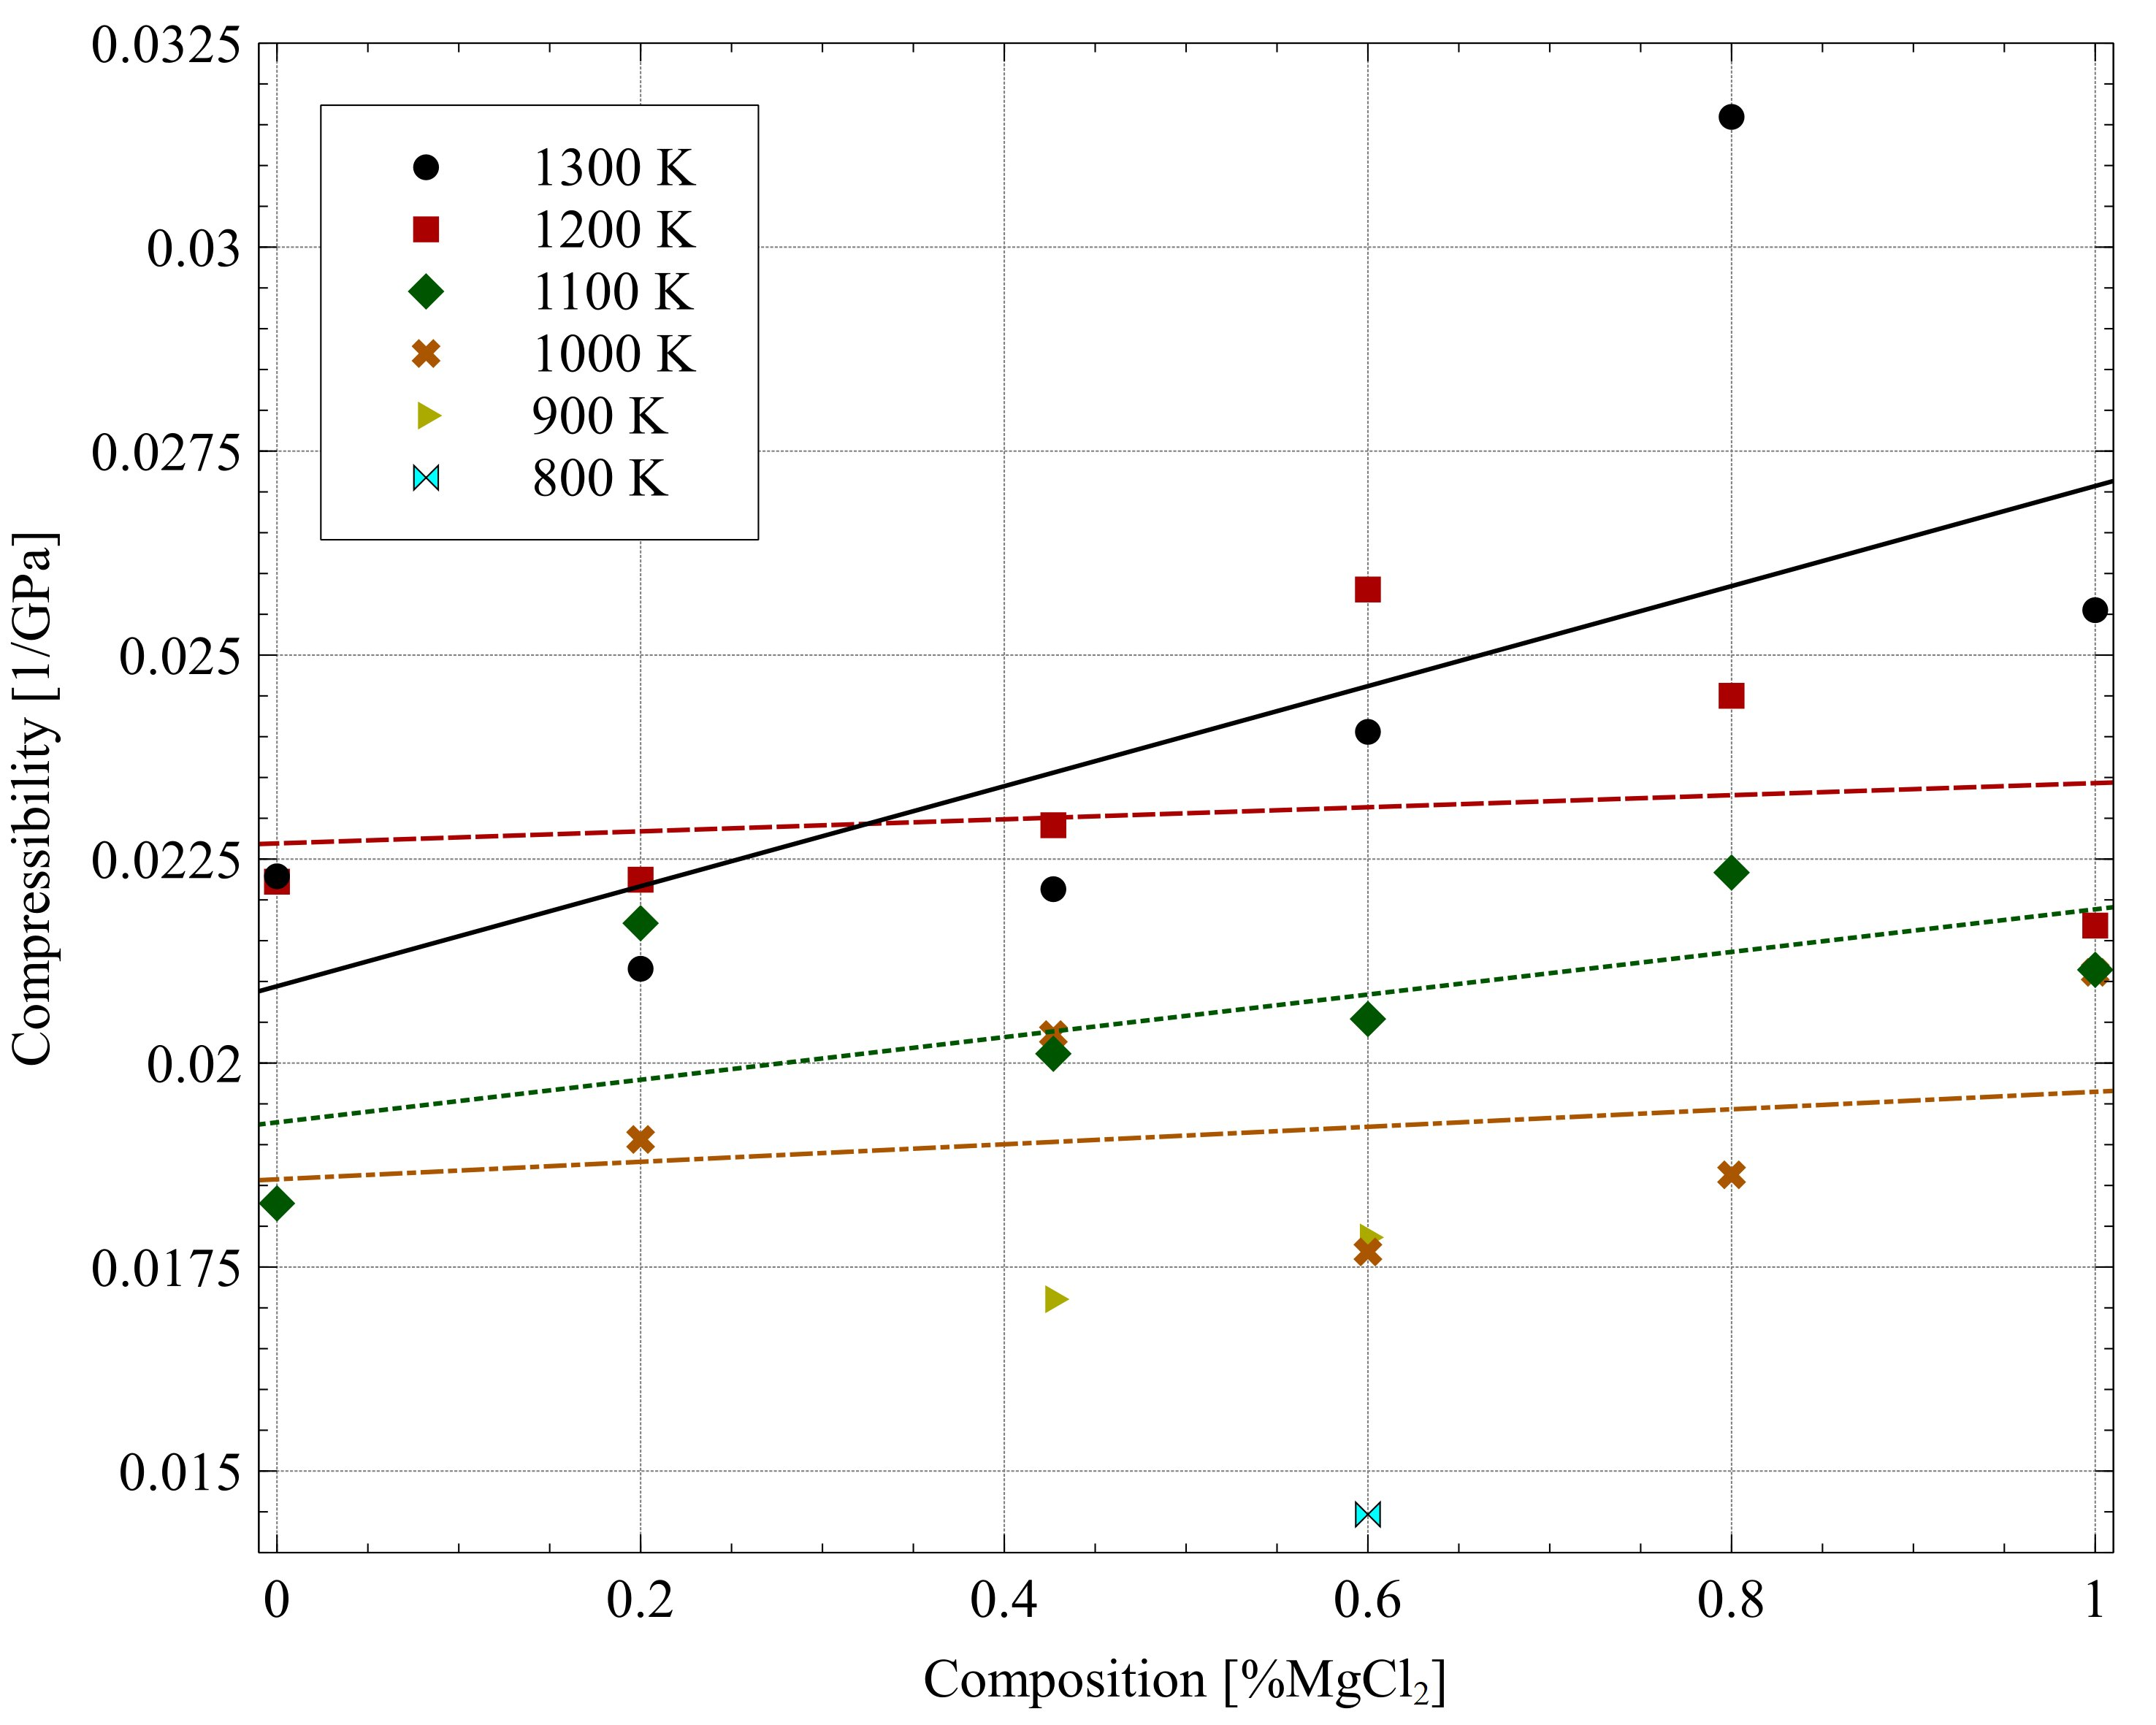
\includegraphics[width=0.7\textwidth]{images/compressibility.jpg} 
 \caption{The compressibility of the NaCl-MgCl$_2$ system as a function of composition and temperature. Linear fits to each complete data set are shown as lines to better illustrate the trends in the data. }
 \label{fig:compressibility}
\end{figure} 

\FloatBarrier



The total energy as a function of temperature for each composition is shown below in Fig. \ref{fig:energy}, illustrating the linear dependence of the energy on temperature. The isobaric heat capacity values calculated from the slope of these curves is shown in Table \ref{table:cp}. There are two observable trends, the first is that heat capacity is constant over these temperature ranges as the relationship between total energy and temperature has a constant slope, and the second is that as the system becomes more MgCl$_2$ rich the heat capacity tends to increase. This increase is monotonic and nearly uniform, with an increase in the heat capacity of approximately 2.85 J/mol-K per 10 molecular percent MgCl$_2$. There are no experimental studies for the heat capacity of NaCl-MgCl$_2$ against which to compare, but there is a study on NaCl-KCl-MgCl$_2$ with mole percent ratios of 27.50\%-32.50\%-40\% conducted by Rincon \cite{del2020experimental}. There is very good agreement with the heat capacity value of 1.090 $\pm$ 0.070 J/g-K compared to our eutectic value of 1.011 J/g-K.

\begin{figure}[h]
 \centering
 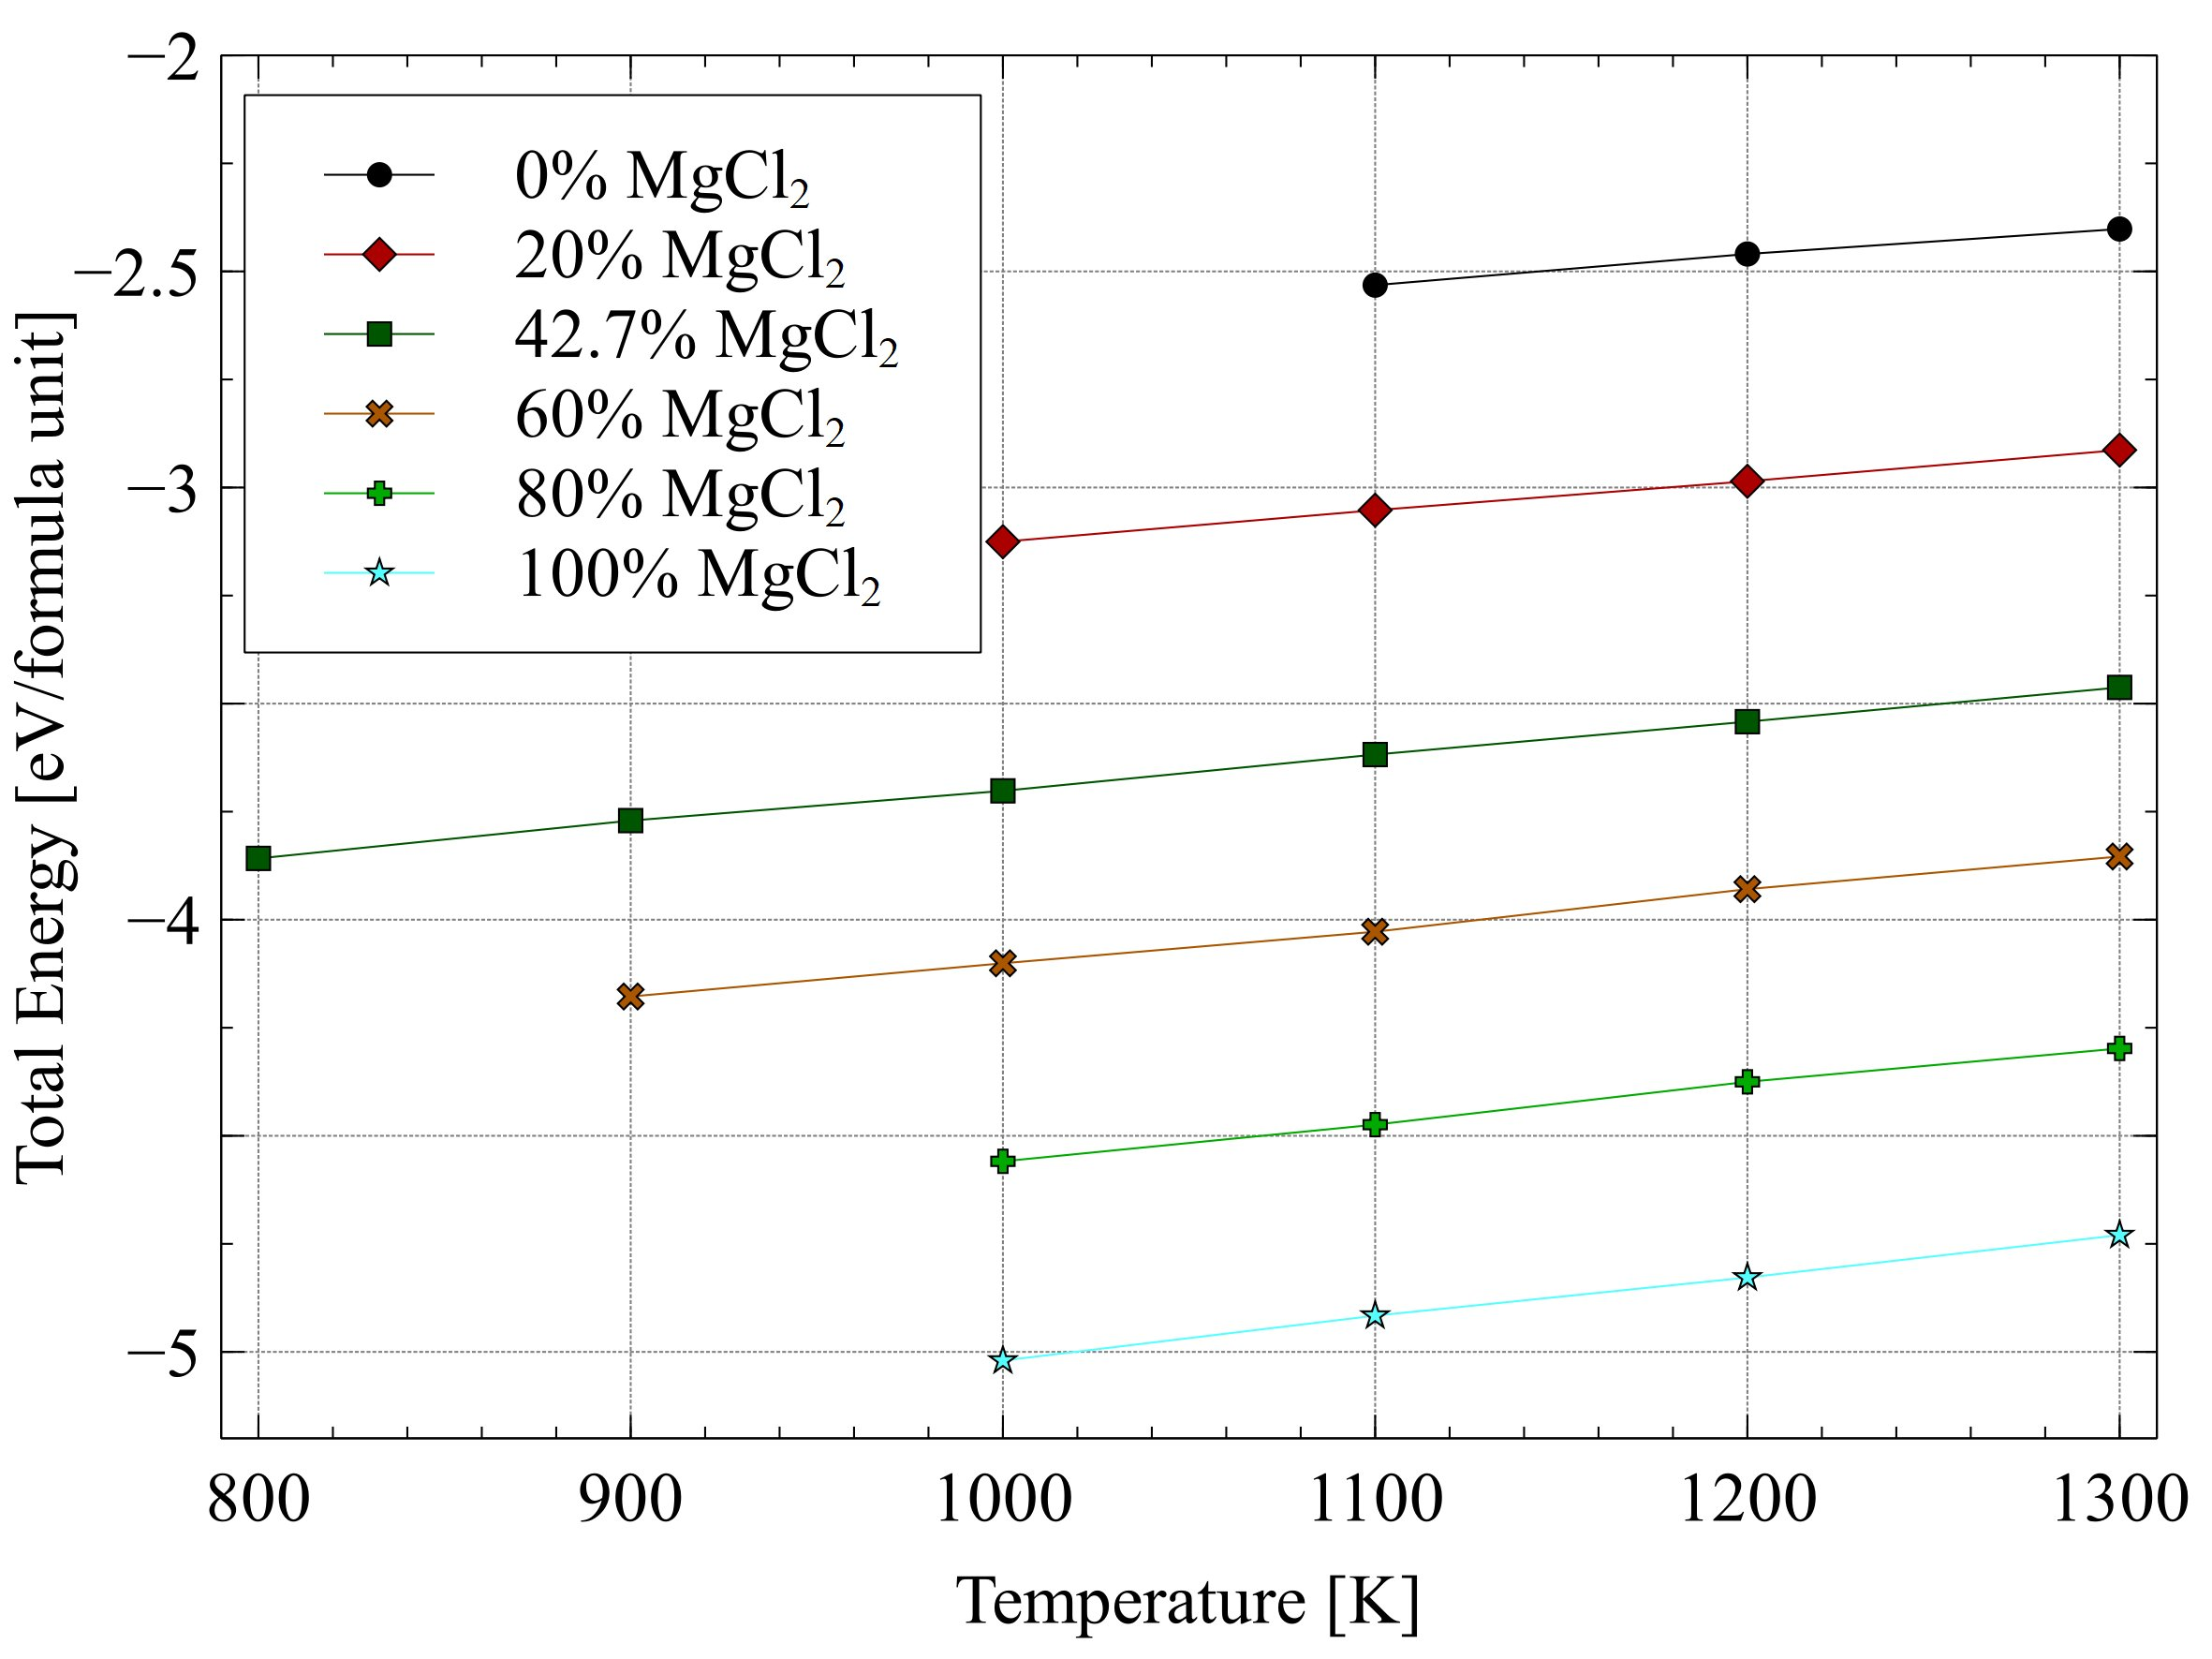
\includegraphics[width=0.8\textwidth]{images/energy.jpg} 
 \caption{The total energy per formula unit for the NaCl-MgCl$_2$ system as a function of temperature at six unique compositions.}
 \label{fig:energy}
\end{figure}

\begin{table}[h!]
\centering
\caption{The isobaric heat capacity for the NaCl-MgCl$_2$ system. Compositions are given in mol percent and heat capacities are given in J/mol-K.}

\begin{tabular}{|c|c|}
\hline
\% MgCl$_2$ &  C$_p$\\
\hline
0  &  62.6\\
20 &  67.1  \\
42.7  &  75.0  \\
60 &  84.0  \\
80 &  85.1  \\
100 &  89.9  \\
\hline
\end{tabular}
\label{table:cp}
\end{table}

The enthalpy of mixing per molecule for the NaCl-MgCl$_2$ system can be seen in Fig. \ref{fig:enthalpy}, where negative values (lower formation energies) indicate the stability of the system. The most stable composition is at the lowest energy which is at the eutectic composition, as expected. This work is over-predicting the enthalpy of mixing by an average of 20.6\% when compared to the experimental data from Karakaya and Thompson \cite{karakaya1986thermodynamic}, but matches the compositional trends. It should be noted that this is the only experimental results with which to compare, and the authors did not provide errors bars to accompany their data. The first order Redlich-Kister expansion was also applied to the enthalpy of mixing and the corresponding fit is illustrated in Fig. \ref{fig:enthalpy}B at 1100 K, and the parameters are given in Table \ref{table:RK_en}. The average percent difference between the Redlich-Kister expansion and the simulation data was 11.3\%, indicating a slightly worse first-order accuracy of the fit than was achieved for the density, but a sufficiently good fit to reproduce the trends in the enthalpy of mixing as a function of temperature.

\begin{figure}[h]
 \centering
 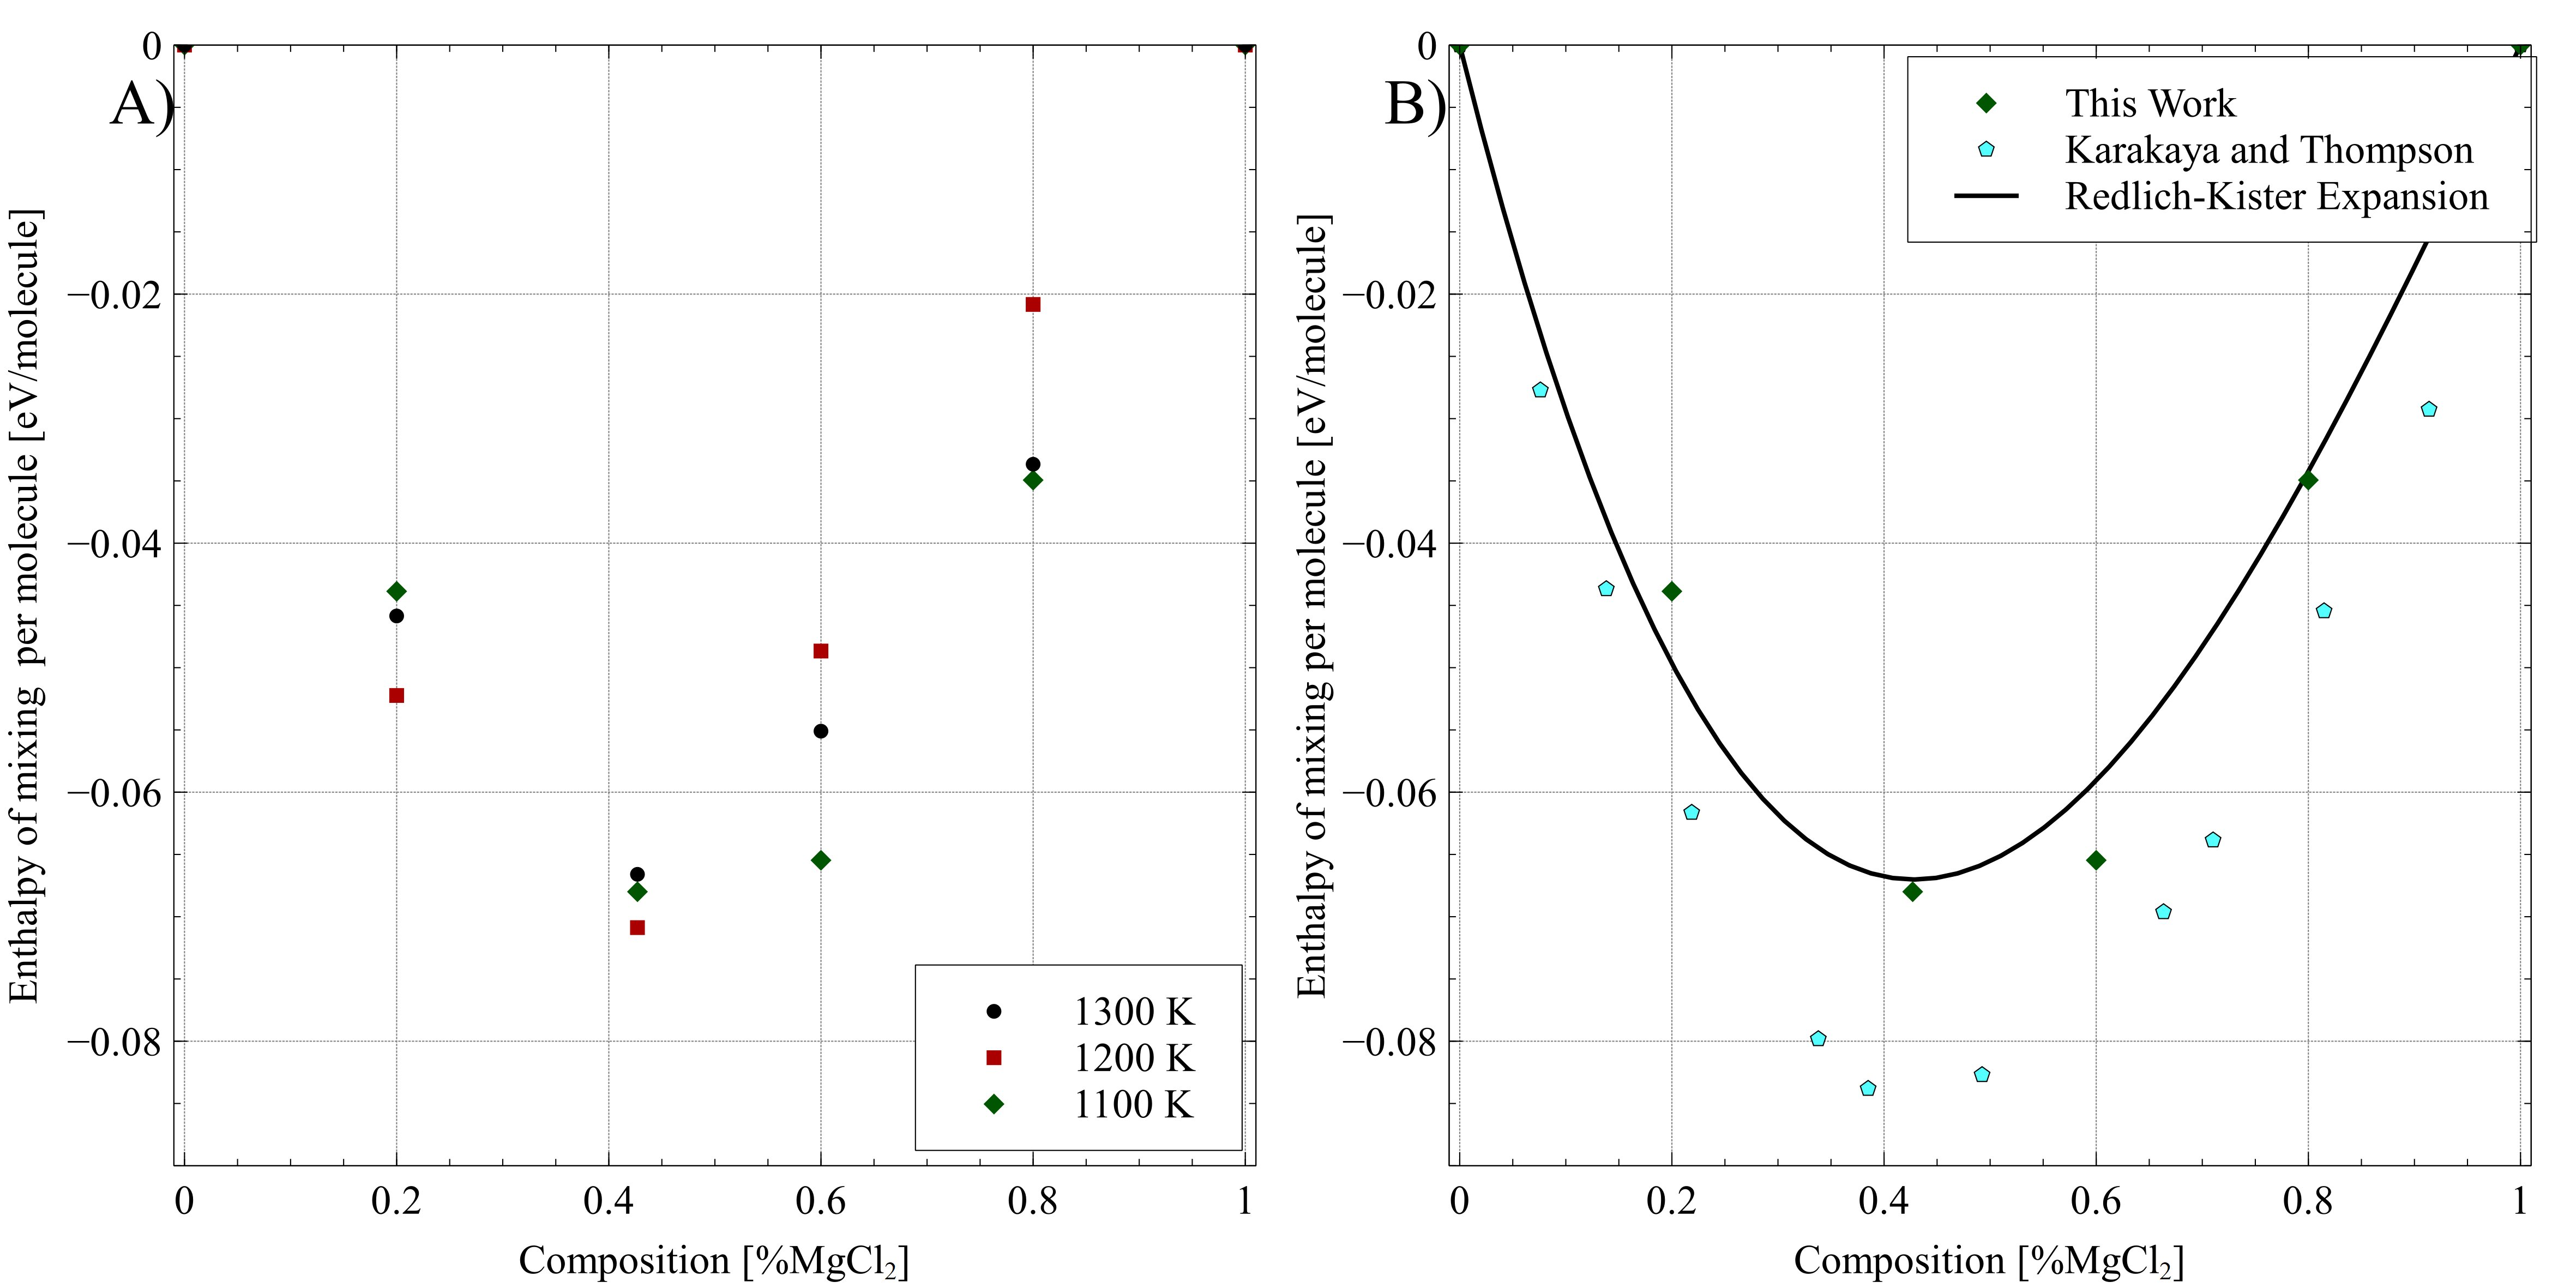
\includegraphics[width=1.0\textwidth]{images/enthalpy.jpg} 
 \caption{A) The enthalpy of mixing per molecule of NaCl-MgCl$_{2}$ for the NaCl-MgCl$_{2}$ system as a function of composition at three temperatures. B) Comparison to experimental measurements at 1073 K \cite{karakaya1986thermodynamic} with the Redlich-Kister expansion fit to the simulation data at 1100 K.}
 \label{fig:enthalpy}
\end{figure} 

\begin{table}[]
\centering
\caption{Redlich-Kister expansion parameters to describe the enthalpy of mixing of the NaCl-MgCl$_2$ system from 1100 K to 1300 K.}
\begin{tabular}{|c|c|c|}
\hline
Parameter &1 & 2 \\
\hline

A	& 0.34782862    & -0.09875289\\
B	  & 7.78757965x10$^{-05}$   & 1.62804955x10$^{-04}$\\
\hline
\end{tabular}
\label{table:RK_en}
\end{table}

The coefficient of thermal expansion is calculated and displayed in Fig. \ref{fig:CTE}. What can be observed is that as the system becomes more MgCl$_2$ rich the thermal expansion decreases. It should be emphasized that for each individual point in Fig. \ref{fig:CTE}, the reference temperature/volume is unique, depending upon the lowest temperature investigated, as indicated in Fig. \ref{fig:density}. The thermal expansion is then calculated from the slope of the volume with respect to the temperature for the entire temperature range and is then divided by the reference volume.  There is good agreement with another AIMD study on the eutectic composition with an NPT ensemble \cite{XU2020568}, where they determined a value of 2.32$\times$10$^{-4}$ K$^{-1}$ at 863 K, while this work finds a value of 2.27$\times$10$^{-4}$ K$^{-1}$, taken over the entire temperature range from 800 K to 1300 K. 

\begin{figure}[h]
 \centering
 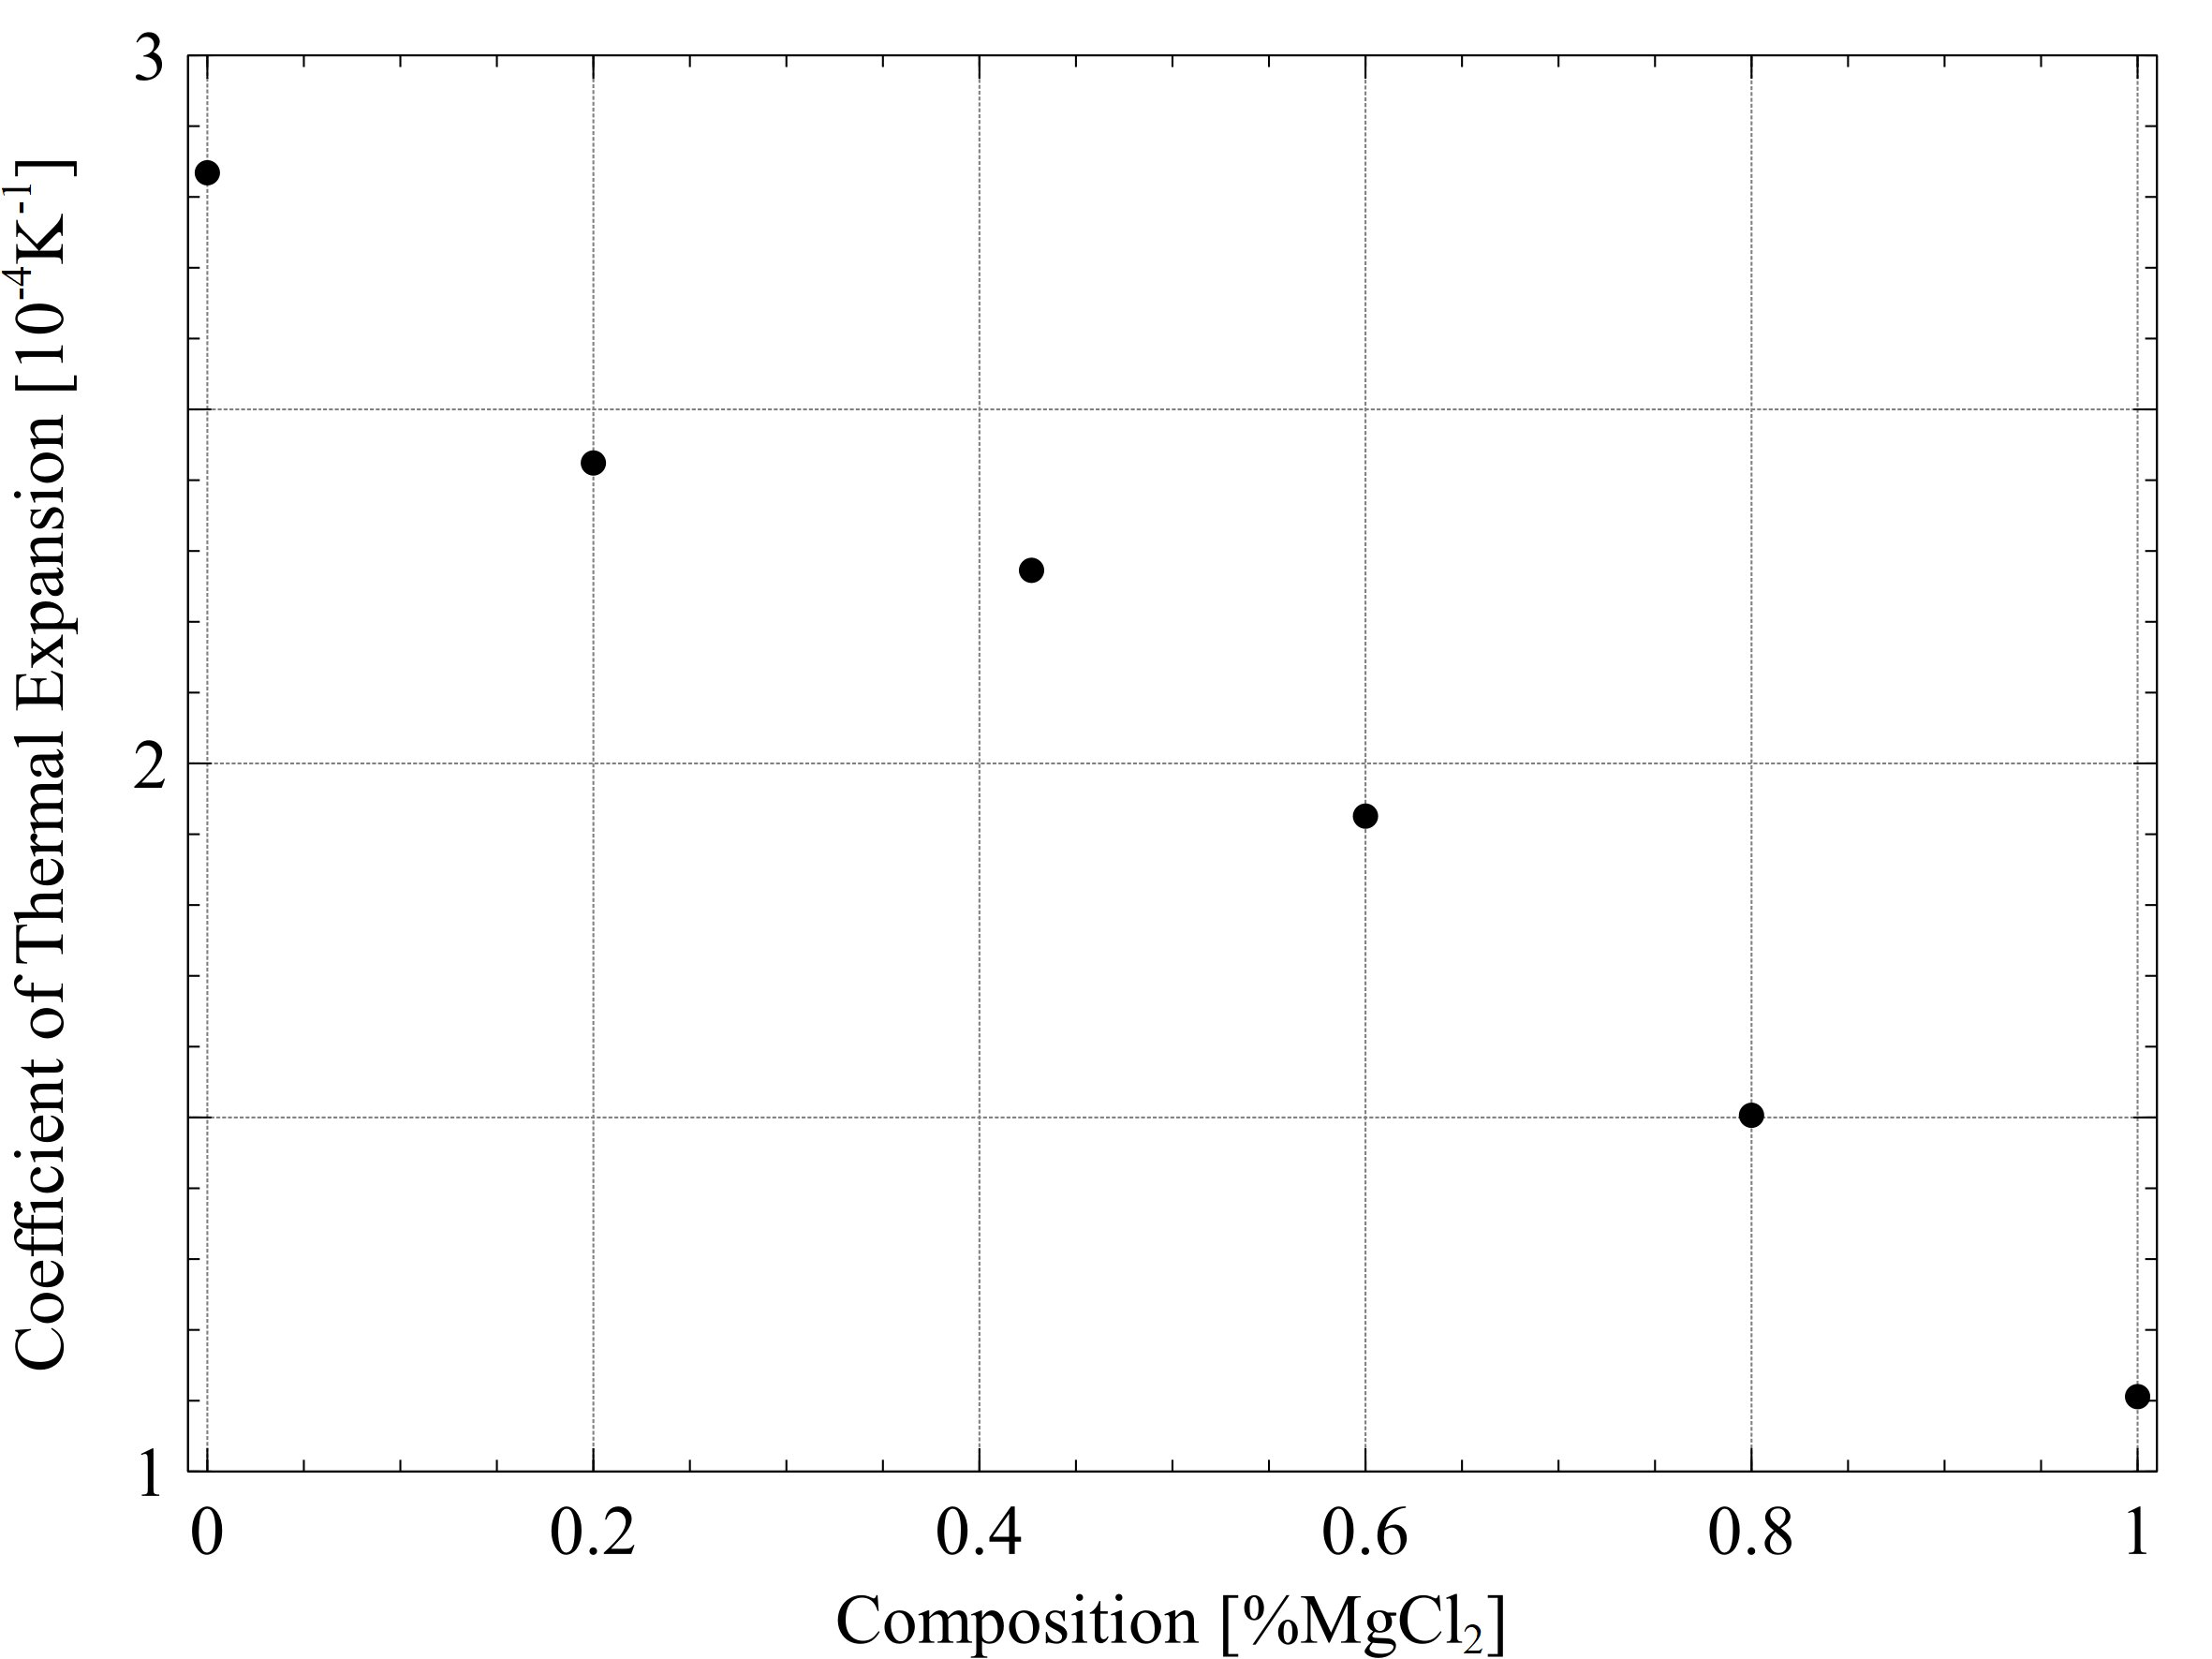
\includegraphics[width=0.8\textwidth]{images/CTE.jpg} 
 \caption{The coefficient of thermal expansion for the NaCl-MgCl$_{2}$ system as a function of composition.}
 \label{fig:CTE}
\end{figure} 
\FloatBarrier

\section{Conclusions}
In this study, the structural and thermophysical properties of NaCl-MgCl$_2$ across the full compositional spectrum have been determined through \textit{ab initio} molecular dynamics. The calculated values for structural properties are in good agreement with the limited experimental literature. The density exhibits excellent agreement with literature values, including a relatively strong deviation from ideal mixing. A Redlich-Kister expansion of the first order was utilized to accurately fit the variation in the density with composition above 1100 K. For the first time, a transition was identified where a monotonic increase of the density with respect to MgCl$_2$ composition occurs above 1100 K. At 1100 K and below, the density of NaCl-80\%MgCl$_2$ is greater than that of MgCl$_2$. Utilizing the computationally determined densities, the compressibility, isobaric heat capacity, and the volumetric thermal expansion coefficient were determined and are in agreement with the limited computational data in the literature. The enthalpy of mixing was determined and over-predicts the single experimental literature value by around 20.6\%, but accurately reproduces the compositional variation, including a minimum at the eutectic composition. This paper provides the most thorough computational analysis of the structural and thermophysical properties of the pseudo-binary NaCl-MgCl$_2$ system to date and can serve to inform thermophysical property databases on molten salts, thermochemical modeling, and computational fluid dynamical studies of salt flow. 


\section{Acknowledgements}

This material is based upon work supported under an University Nuclear Leadership Program Graduate Fellowship. This work is also supported through the INL Laboratory Directed Research and Development (LDRD) Program under DOE Idaho Operations Office Contract DE-AC07-05ID14517. This research made use of the resources of the High-Performance Computing Center at Idaho National Laboratory, which is supported by the Office of Nuclear Energy of the U.S. Department of Energy and the Nuclear Science User Facilities.  

\bibliography{reference}
%\end{multicols}

\end{document}
